% =====================================================================
%  When Does Policy Switching Beat the Best Static Policy?
%  A Reproducible Ceiling Study (IEEE Q1 Journal Revision)
%  Build: python3 build.py   (fills bibliography, then pdflatex x2)
% =====================================================================
\documentclass[10pt,twocolumn]{article}
\usepackage[T1]{fontenc}
\usepackage[utf8]{inputenc}
\usepackage{mathptmx}
\usepackage[letterpaper,top=0.75in,bottom=0.85in,left=0.65in,right=0.65in,columnsep=0.22in]{geometry}
\usepackage{amsmath,amssymb,booktabs,multirow,graphicx,xcolor,microtype,cite,url,array,enumitem,titlesec,balance}
\usepackage[font=footnotesize,labelfont=bf,labelsep=period,justification=justified,singlelinecheck=false]{caption}
\usepackage[colorlinks=true,allcolors=blue!50!black,breaklinks=true]{hyperref}
\usepackage{xr}
\externaldocument[S-]{supplement}
\urlstyle{rm}

% ---- IEEE-like headings and floats ----------------------------------
\renewcommand{\thesection}{\Roman{section}}
\renewcommand{\thesubsection}{\thesection-\Alph{subsection}}
\titleformat{\section}{\centering\normalfont\small\scshape}{\thesection.}{0.6em}{}
\titleformat{\subsection}{\normalfont\small\itshape}{\Alph{subsection}.}{0.6em}{}
\titlespacing*{\section}{0pt}{9pt plus 2pt minus 2pt}{4pt}
\titlespacing*{\subsection}{0pt}{6pt plus 2pt minus 1pt}{2pt}
\renewcommand{\figurename}{Fig.}
\renewcommand{\tablename}{Table}
\renewcommand{\thetable}{\Roman{table}}
\captionsetup[table]{labelsep=newline,justification=centering,textfont=sc,labelfont=sc,singlelinecheck=true}
\captionsetup[figure]{justification=justified}
\setlength{\textfloatsep}{8pt plus 2pt minus 2pt}
\setlength{\floatsep}{8pt plus 2pt minus 2pt}
\setlength{\intextsep}{8pt plus 2pt minus 2pt}
\setlength{\parindent}{1.2em}
\setlist{nosep,leftmargin=1.4em}
\renewcommand{\arraystretch}{1.08}
\pagestyle{plain}
\sloppy

\newcommand{\us}{\ifmmode\,\mathrm{\mu s}\else\,\textmu s\fi}
\newcommand{\Cs}{C_{s}}
\newcommand{\Dw}{D_{w}}
\newcommand{\code}[1]{\path{#1}}
\hypersetup{pdftitle={When Does Policy Switching Beat the Best Static Policy? A Reproducible Ceiling Study},
            pdfauthor={M. Qasim, H. Tahir, H. Ahmad, M. G. Ghouri}}

\begin{document}

\twocolumn[
\begin{center}
{\LARGE When Does Policy Switching Beat the Best Static Policy?\\\medskip
         A Reproducible Ceiling Study\par}
\vspace{8pt}
{\large Muhammad Qasim, Hunain Tahir, Hussain Ahmad, and Mohsin Ghaffar Ghouri\par}
\vspace{3pt}
{\footnotesize University of Management and Technology (UMT), Lahore, Pakistan.\\ M.\ Qasim is also with the Anoneurx Research Lab.\\
Corresponding author: M.\ Qasim (e-mail: itskashie@anoneurx.com)\par}
\end{center}
\vspace{6pt}
]

% =====================================================================
% ABSTRACT
% =====================================================================
\noindent{\small\bfseries\itshape Abstract---}{\small\bfseries
Discrete policy switching is a recurring design pattern in adaptive cache and page replacement: monitor a workload for drift, rank candidate policies in shadow caches, and switch when a candidate outperforms the incumbent. We bound the achievable headroom of discrete switching using an exact Viterbi dynamic-programming (DP) hindsight oracle under an \emph{independent-replay model} across 88 traces (30 workload families), 21 baseline policies, and cache capacities from $1\%$ to $50\%$ of working-set size (WSS). At an assumed full-refill penalty ($c_{\text{switch}}=C$, $W=50{,}000$), \textbf{0 of 90} family--capacity groups ($1\%$--$10\%$ WSS) clear a $0.02$ net miss-ratio reduction (trace-weighted mean $0.0000$, family-macro mean $0.0000$, 4-source mean $0.0000$, max $0.0021$); across all $440$ pairs ($1\%$--$50\%$ WSS), \textbf{0 of 440} clear $0.02$. Under assumed lower migration penalties ($c_{\text{switch}} \le 0.10C$) and fine windows ($W=5{,}000$), $13/264$ pairs ($4.9\%$) clear $0.02$, and $0/264$ clear $0.02$ once $c_{\text{switch}} \ge 0.50C$ across $W \in \{5\text{k},10\text{k},25\text{k},50\text{k}\}$. We also evaluate 17 online switching controllers and 4 shadow ablations after fixing a capacity-overrun bug ($|S|+|M|>C$ under ghost hits) discovered via independent cross-validation in our initial \code{S3-FIFO} implementation; \code{LRU}, \code{FIFO}, \code{ARC}, and \code{SIEVE} matched reference implementations bit-for-bit. Across $1\%$--$10\%$ WSS, static \code{CAR} ($0.5151$) and \code{S3-FIFO} ($0.5167$) achieve the lowest global mean miss ratios, and all 17 online controllers incur $+0.0109$ to $+0.0165$ higher mean miss ratio than \code{S3-FIFO} (family-level $n=30$ Holm-adjusted $p=1.000$, $r_b \in [+0.11, +0.39]$). Cold-window shadow evaluation mis-ranks the top-1 policy in $54.9\%$ of evaluation windows, and an exploratory leak-free leave-one-family-out ranker achieves $\text{AUC}=0.927$ ($\text{PR-AUC}=0.573$) but $0.525$ balanced accuracy ($F_1=0.125$) on $13/88$ positives.\par}

\vspace{4pt}
\noindent{\small\bfseries\itshape Index Terms---}{\small page replacement, cache replacement, drift detection, policy switching, hindsight oracle, measurement study\par}
\vspace{6pt}

% =====================================================================
\section{Introduction}
\label{sec:intro}
% =====================================================================

Page and cache replacement determines which blocks remain resident when memory is constrained. Because real workloads alternate among sequential scans, hot-object reuse, and random I/O, no single static eviction rule is optimal in every interval. This observation has motivated decades of adaptive replacement designs, from SEQ~\cite{seq} and EELRU~\cite{eelru} to ARC~\cite{arc}, LeCaR~\cite{lecar}, CACHEUS~\cite{cacheus}, and recent learning-augmented policies~\cite{lrb,l3cache,s4fifo}.

A recurring architecture in this literature is \emph{discrete policy switching}: monitor the miss stream for workload drift, evaluate a pool of candidate policies via sampled shadow caches, and switch the active policy when a candidate outperforms the incumbent. Each transition incurs metadata migration or cache warm-up overhead, while the hoped-for benefit is a lower miss ratio in the new regime. Whether that benefit exceeds transition costs---especially against modern scan-resistant static baselines such as S3-FIFO~\cite{s3fifo} and SIEVE~\cite{sieve}---is rarely bounded explicitly.

We ask one concrete question: \emph{when, if ever, does discrete policy switching beat the best static policy once switching costs are counted?} Rather than proposing a new switching controller, we compute a Viterbi dynamic-programming (DP) hindsight oracle under an \emph{independent-replay model} across 88 traces and compare it against both the per-pair best static policy and the global best static policy. We also evaluate 17 online switching controllers, diagnose shadow-ranking failures, test whether workload features predict rare switching headroom, and report a complete independent simulator validation audit.

\textbf{Contributions.}
\begin{enumerate}
\item \textbf{Model-Relative Oracle Ceiling:} An exact Viterbi DP ceiling under independent replay across 88 traces ($1\%$--$50\%$ WSS), 9 normalized switch-cost fractions ($c_{\text{switch}} \in [0,C]$), and 4 window sizes ($W \in \{5\text{k},10\text{k},25\text{k},50\text{k}\}$), plus aggregation-sensitivity checks across trace-, family-, source-, and non-stationary-weighted averages.
\item \textbf{Mathematical Characterization \& Counterexample:} Exact proof of DP optimality within the independent-replay model alongside a constructive $C=2$ counterexample demonstrating that independent replay is \emph{not} a universal upper bound on arbitrary finite-cache state-carrying executions.
\item \textbf{Simulator Validation \& Bug Remediation:} Bit-for-bit cross-validation of \code{LRU}, \code{FIFO}, \code{ARC}, and \code{SIEVE} against independent reference implementations (\code{0} miss difference), paired with discovery, remediation, and full 88-trace re-execution of a capacity-overrun bug (\code{|S|+|M| > C}) in our initial \code{S3-FIFO} implementation.
\item \textbf{Cluster-Aware Controller Evaluation \& Failure Diagnosis:} A matched comparison of 17 online controllers plus 4 shadow ablations and a 21-policy expansion (\code{ContShadow-21}) using family-level ($n=30$) cluster inference, direct shadow-ranking accuracy across $9{,}564$ windows, and 50-trial \code{switchTo()} migration latency measurements.
\item \textbf{Exploratory Screening \& Reproducible Artifact:} A leak-free leave-one-family-out (LOFO) screening analysis separating ranking ($\text{AUC}=0.927$) from binary classification ($F_1=0.125$), together with a public artifact and full audit reports.
\end{enumerate}

% =====================================================================
\section{Background and Related Work}
\label{sec:related}
% =====================================================================

Adaptive cache replacement spans three paradigms: (i)~continuous internal adaptation, such as ARC~\cite{arc}, CAR~\cite{car}, and DIP set-dueling~\cite{dip}; (ii)~online expert weighting (Hedge~\cite{hedge}) over two policies, as in ACME~\cite{acme02}, LeCaR~\cite{lecar}, and CACHEUS~\cite{cacheus}; and (iii)~epoch-based discrete policy switching driven by drift detectors (CUSUM~\cite{page}, Page--Hinkley~\cite{page}, ADWIN~\cite{adwin}, Gama et al.~\cite{gama}) and sampled shadow caches (SHARDS~\cite{shards}, miniature simulations~\cite{mini}, Acme~\cite{acme}). Recent learned and learning-augmented policies---including Hawkeye~\cite{hawkeye}, LRB~\cite{lrb}, 3L-Cache~\cite{l3cache}, LPR~\cite{lpr}, EACLOCK~\cite{eaclock}, Clock2Q+~\cite{clock2q}, and S4FIFO~\cite{s4fifo}---target single-policy robustness, while S3-FIFO~\cite{s3fifo} and SIEVE~\cite{sieve} demonstrate that lightweight FIFO-based scan resistance rivals complex adaptive structures. Large-scale studies such as Twitter's cache analysis~\cite{twitter} motivate evaluating across diverse workload regimes, and emerging GPU/eBPF memory schedulers~\cite{msched,gpuext} revive interest in runtime policy selection. Unlike prior controller proposals, our work provides an empirical ceiling study bounded by an independent-replay DP oracle and a cluster-aware failure diagnosis of discrete switching.

% =====================================================================
\section{Problem Formulation}
\label{sec:problem}
% =====================================================================

Let a trace be a sequence of page references $r_1, \dots, r_N$ with working-set size $\text{WSS} = |\{r_1,\dots,r_N\}|$ and cache capacity $C = \max(1, \operatorname{round}(f \cdot \text{WSS}))$ for capacity fraction $f \in \{0.01, 0.05, 0.10, 0.25, 0.50\}$. After a warm-up prefix of $N_{\text{warm}} = \min(100{,}000, \lfloor 0.1 N \rfloor)$ references, the remaining $N_{\text{eval}} = N - N_{\text{warm}}$ references are partitioned into $T = \lfloor N_{\text{eval}} / W \rfloor$ complete windows of length $W$ (trailing incomplete references $N_{\text{eval}} \bmod W$ are omitted so every window has equal weight).

We distinguish four quantities across a policy pool $\mathcal{P}$ ($|\mathcal{P}|=21$):
\begin{itemize}
\item \textbf{Best Global Static Policy:} The single policy $p_{\text{glob}}^* \in \mathcal{P}$ minimizing mean miss ratio across all $(i, f)$ pairs (here \code{CAR} at $0.5151$, closely followed by \code{S3-FIFO} at $0.5167$, which serves as the fixed-capacity controller baseline).
\item \textbf{Per-Pair Best Static Policy:} $p_{i,f}^* = \arg\min_{p \in \mathcal{P}} \text{MR}_{i,f,p}$, chosen ex post for each trace--capacity pair. By Jensen's inequality, $\mathbb{E}[\min_p \text{MR}_{i,f,p}] \le \min_p \mathbb{E}[\text{MR}_{i,f,p}]$.
\item \textbf{Independent-Replay Hindsight Oracle:} The minimum-cost schedule $(p_1,\dots,p_T) \in \mathcal{P}^T$ computed over independently replayed per-window miss counts $m_{t,p}$ with fixed transition penalty $c_{\text{switch}}$.
\item \textbf{State-Carrying Switching Execution:} Executing a schedule $(p_1,\dots,p_T)$ in a single live cache where switching at window boundaries transfers resident page IDs and coarse recency/frequency metadata via \code{switchTo()}.
\end{itemize}

Our primary confirmatory hypotheses (recorded locally in git before running the study, without external third-party preregistration and hence treated as post hoc) tested: \textbf{H1}, whether the oracle clears a $0.02$ net miss-ratio gain on $\ge 2/3$ of traces in any family--capacity group; \textbf{H2}, whether any online controller beats the best static baseline; and \textbf{H3} (exploratory), whether trace features predict zero-cost headroom on unseen families.

% =====================================================================
\section{Mathematical Model}
\label{sec:model}
% =====================================================================

Under the independent-replay model, each policy $p \in \mathcal{P}$ processes the full trace $[1, N_{\text{warm}} + TW]$ with its own warm cache state, producing integer per-window miss counts $m_{t,p} \in \{0,\dots,W\}$ for $t = 1,\dots,T$. Given normalized switch penalty $c_{\text{switch}} = \beta C$ ($\beta \in [0, 1]$, measured in miss-equivalents), the Viterbi dynamic program solves:
\begin{align}
\text{dp}[1][p] &= m_{1,p}, \label{eq:dp_init}\\
\text{dp}[t][p] &= m_{t,p} + \min_{q \in \mathcal{P}} \Bigl(\text{dp}[t-1][q] + c_{\text{switch}} \cdot \mathbf{1}[p \ne q]\Bigr), \label{eq:dp_rec}
\end{align}
for $t = 2,\dots,T$. Initial policy selection at $t=1$ is free. Ties in $\text{stay} \le \text{switch}$ break in favor of staying ($\mathbf{1}[p \ne q]=0$) to avoid zero-gain switches. Using running best and second-best predecessors $(q_1, q_2)$ per window, \eqref{eq:dp_rec} runs in $\mathcal{O}(TP)$ time and $\mathcal{O}(TP)$ space. Defining $S = \sum_{t=2}^T \mathbf{1}[p_t^* \ne p_{t-1}^*]$, the oracle objective ratio is $J^* = (\sum_{t=1}^T m_{t,p_t^*} + S \cdot c_{\text{switch}}) / (TW)$, and the net gain over the per-pair best static policy is $g(c_{\text{switch}}) = \text{MR}(p_{i,f}^*) - J^*$.

\textbf{Necessary break-even condition (Proposition 1).} Suppose a switch enters a dwell segment of $L \in \{1,\dots,T-1\}$ consecutive windows ($L \cdot W$ references) and pays $c_{\text{switch}}$ miss-equivalents. Let $\Delta M = \sum_{t \in \text{dwell}} (m_{t,p^*} - m_{t,p_t^*})$ be the cumulative miss reduction over the dwell and $\overline{\Delta m} = \Delta M / (L \cdot W)$ be the mean per-window miss-ratio reduction. Positive net gain requires $\Delta M > c_{\text{switch}}$, i.e.:
\begin{equation}
\overline{\Delta m} > \frac{c_{\text{switch}}}{W \cdot L} = \frac{\beta C}{W \cdot L}. \label{eq:breakeven}
\end{equation}
Across $S$ switches over $T$ windows, positive trace-wide net gain requires $\sum_{t=1}^T (m_{t,p^*} - m_{t,p_t^*}) > S \cdot c_{\text{switch}}$. For $c_{\text{switch}} = C = 5{,}000$, $W = 50{,}000$, and $L=1$, breaking even requires $>10\%$ miss-ratio reduction in a single window.

\textbf{What the model does and does not establish (and counterexample).} Within the independent-replay model (where every candidate maintains an un-sampled warm cache and switching transfers that warm state at cost $c_{\text{switch}}$), \eqref{eq:dp_init}--\eqref{eq:dp_rec} is exact. However, independent replay at $c_{\text{switch}}=0$ is \emph{not} a universal mathematical lower bound on misses for arbitrary finite-cache state-carrying executions. Because finite-cache policies are non-additive under state perturbations, consider $C=2$ with $r^{(1)}=(1,2,3,4)$ and $r^{(2)}=(1,4,5,4,5)$: independent-replay DP($c=0$) over $\{\text{MRU},\text{LRU}\}$ incurs $\min(4,4)+\min(3,2)=6$ misses, whereas state-carrying \code{MRU} $\to$ \code{LRU} inherits $\{1,4\}$ from $r^{(1)}$ and incurs $4+1=5$ misses. On realistic phase-shifting workloads, however, ghost-state loss causes state-carrying execution to incur substantially \emph{more} misses than independent replay (Section~\ref{sec:validation}). Thus, $g(c_{\text{switch}})$ is an exact model-relative ceiling and an optimistic empirical benchmark whenever cold/ghost transition penalties are at least $c_{\text{switch}}$.

% =====================================================================
\section{Experimental Methodology}
\label{sec:method}
% =====================================================================

All experiments run in a single-file C++17 simulator (\code{src/pathA_sim.cpp}, 1,902 lines) implementing 21 policies: \code{S3-FIFO}~\cite{s3fifo}, \code{SIEVE}~\cite{sieve}, \code{ARC}~\cite{arc}, \code{CAR}~\cite{car}, \code{LIRS}~\cite{lirs}, \code{W-TinyLFU}~\cite{wtinylfu}, \code{2Q}~\cite{twoq}, \code{CLOCK-Pro}~\cite{clockpro}, \code{LeCaR}~\cite{lecar}, \code{CACHEUS}~\cite{cacheus}, \code{LHD}~\cite{lhd}, \code{DIP-set-duel}~\cite{dip}, \code{LPR-style}~\cite{lpr}, \code{3L-style}~\cite{l3cache}, \code{MGLRU-style}~\cite{mglru}, \code{LRB-style} (online SGD~\cite{lrb}, seed \code{4242}), \code{LRU}, \code{FIFO}, \code{CLOCK}, \code{LFU-A}, and \code{MRU} (compared against Belady-inspired oracle bounds~\cite{belady}).

We evaluate 17 online switching controllers over a 6-policy pool (\code{LRU}, \code{LFU-A}, \code{2Q}, \code{MRU}, \code{S3-FIFO}, \code{ARC}): 3 budgets (low/med/high) each for \code{CUSUM} ($h\in\{8,5,3\}$), \code{Page-Hinkley} ($\lambda\in\{9,5,2\}$), \code{ADWIN} ($\delta\in\{2\times 10^{-4},2\times 10^{-3},2\times 10^{-2}\}$), \code{Periodic} ($40,20,10$ epochs), and \code{Random} ($p_{\text{trig}}\in\{0.025,0.05,0.10\}$, seed \code{99}), plus \code{OracleTrig} (oracle switch boundaries) and \code{ContShadow} (every 10 epochs). Epoch length is $2{,}000$ references; shadow caches sample $20\%$ by page hash with $\Cs = \min(\lfloor 0.2C\rceil, \max(8,\lfloor 0.5\Dw\rceil))$, $40\%$ shadow warm-up, and $z=1.28$ lower-confidence-bound selection over 4 sub-blocks. In \code{switchTo()}, resident page IDs sorted by last access timestamp and access counts are loaded into the new policy; policy-specific ghost lists (\code{S3-FIFO} ghost, \code{ARC} $B_1/B_2$, \code{2Q} $A_{1\text{out}}$) cannot be preserved across heterogeneous policies. We also test 4 shadow ablations (\code{FullShadow}, \code{FullShadow-CostAware}, \code{PersistentShadow}, \code{PersistentShadow-CostAware} with $p=1.0, \Cs=C$) and \code{ContShadow-21} (all 21 policies).

\textbf{Switch-cost modeling.} We treat $c_{\text{switch}} = \beta C$ across $\beta \in \{0, 0.02, 0.05, 0.10, 0.15, 0.20, 0.25, 0.50, 1.00\}$ as \emph{assumed normalized miss-equivalent cost scenarios} rather than empirically calibrated hardware penalties, and separately measure actual in-memory \code{switchTo()} migration latency in C++.

% =====================================================================
\section{Dataset and Trace Conversion Methodology}
\label{sec:dataset}
% =====================================================================

We evaluate 88 traces spanning 30 workload families and four sources (Table~\ref{tab:sources}): (i)~10 real-application page traces captured via \code{LD_PRELOAD} (\code{tracer/pc_trace.c} interposing \code{read}/\code{pread}/\code{write}/\code{pwrite}/\code{fread}/\code{fwrite}/\code{mmap} on regular files, mapping 4\,KiB file-page keys; \code{SQLite}, \code{git}, Python ETL; 0.31M--2.29M refs); (ii)~60 instrumented-program page traces across 15 kernels (\code{real_traces.cpp}, logging 4\,KiB virtual addresses, 0.30M refs each, median WSS 3,907); (iii)~12 public FIU block-I/O traces~\cite{fiu,pdl} (0.42M--0.50M refs, median WSS 156,736); and (iv)~6 public PDL storage/cache traces~\cite{pdl,msr,twitter} (1.00M-reference prefixes, median WSS 171,823).

\begin{table}[t]
\centering
\footnotesize
\caption{Trace Corpus Summary (88 Traces, 30 Families)}
\label{tab:sources}
\resizebox{\columnwidth}{!}{\begin{tabular}{lrrrr}
\toprule
Source & Families & Traces & Refs (mean) & WSS (median) \\
\midrule
Real-app page traces (SQLite, git, Python) & 3 & 10 & 0.80M & 6,092 \\
Instrumented programs (15 kernels) & 15 & 60 & 0.30M & 3,907 \\
Public FIU block-I/O traces & 6 & 12 & 0.49M & 156,736 \\
Public PDL cache/storage traces & 6 & 6 & 1.00M & 171,824 \\
\midrule
Total & 30 & 88 & 0.43M & 4,128 \\
\bottomrule
\end{tabular}
}
\end{table}

\textbf{Trace conversion \& comparability.} All sources are normalized to dense \code{uint32_t} IDs in first-touch order. For \code{fiu_public} and \code{pdl_public} (\code{oracleGeneral} 24-byte \code{<IQIq} records), each record emits one reference to \code{ids[oid]}, discarding request size (\code{_sz}) and read/write flags; \code{fiu_*_test} retains global train/test IDs (\code{max_id > wss}). Two structural limitations are audited directly: (1)~instrumented kernels comprise $68.2\%$ of traces and yield only $2$--$5$ windows at $W=50\text{k}$--$100\text{k}$; and (2)~FIU traces exhibit $\ge 31\%$ compulsory first-touch misses. Section~\ref{sec:results} therefore reports trace-weighted, 30-family macro-averaged, 4-source equal-weighted, and non-stationary-only ($g(0)>0.001$, $n=21$ traces) aggregates.

% =====================================================================
\section{Simulator and Oracle Validation}
\label{sec:validation}
% =====================================================================

We implemented both internal validation (\code{tests/validate_simulator.cpp}, \code{tests/run_tests.py}) and independent cross-validation (\code{tests/external_validation/}):
\begin{itemize}
\item \textbf{Hand-worked \& invariant checks:} Exact hit/miss matches for \code{LRU} (10 misses), \code{FIFO} (9 misses), and \code{MRU} (7 misses) on $\{1,2,3,4,1,2,5,1,2,3,4,5\}$ ($C=3$), repeated-reference checks ($C=1,2$), scan resistance, and capacity monotonicity.
\item \textbf{Viterbi DP vs.\ brute force:} Exhaustive $P^T$ enumeration ($P=4, T=5$, $1{,}024$ schedules) matched \code{solveDPOracle()} to $10^{-12}$ across $c_{\text{switch}} \in \{0, 15, 35, 100\}$.
\item \textbf{State-carrying vs.\ independent replay:} On a 3-phase trace ($3\times 2{,}000$ refs, $C=10$: hot $\{0..9\}$ $\to$ cyclic scan $\{100..115\}$ $\to$ hot $\{0..9\}$), independent-replay $c=0$ oracle scored $52$ misses ($0.0087$) whereas state-carrying \code{switchTo()} incurred $2{,}011$ misses ($0.3352$).
\item \textbf{Independent reference cross-validation (Table~\ref{tab:extval}):} Because \code{libCacheSim} was unavailable in our offline environment, we cross-checked \code{LRU}, \code{FIFO}, \code{ARC}, \code{S3-FIFO}, and \code{SIEVE} against independent Python reference implementations across synthetic Zipfian ($\alpha=1.8$, $C=10,50$) and three \code{traces_real/} traces (\code{btree_s101}, \code{hashjoin_s101}, \code{bfs_s101} at $1\%, 5\%, 10\%$ WSS). \code{LRU}, \code{FIFO}, \code{ARC}, and \code{SIEVE} matched \textbf{bit-for-bit} (\code{0} miss difference) across all 11 configurations.
\item \textbf{\code{S3-FIFO} capacity-invariant bug discovery and fix:} Cross-validation initially revealed that \code{S3FIFO} in \code{src/pathA_sim.cpp} violated $|S|+|M|\le C$: during warm-up promotions when $|M|<M_{\text{cap}}$ and on ghost hits inserting into $M$ after evicting from $S$, $|S|+|M|$ grew to $2{,}118$ pages on \code{btree_s101} at $C=1{,}130$ ($1.87\times C$), artificially lowering its miss ratio from $0.2463$ (strict-capacity reference) to $0.1698$. We fixed \code{S3FIFO::evict()} and \code{S3FIFO::access()} to enforce $|S|+|M|\le C$ strictly (verified across adversarial stress tests and Table~\ref{tab:extval}, where \code{pathA\_sim} now matches the strict-capacity reference within $0.00$--$0.09$ percentage points) and re-ran the entire 88-trace study.
\end{itemize}

\begin{table}[t]
\centering
\footnotesize
\caption{Independent Cross-Validation (\texttt{pathA\_sim} Post-Fix vs.\ Reference)}
\label{tab:extval}
\resizebox{\columnwidth}{!}{\begin{tabular}{llrrrr}
\toprule
Trace ($C$) & Policy & \code{pathA\_sim} EvalM & Ref EvalM & Diff & Status \\
\midrule
\code{synth_zipf} (50) & \code{LRU}/\code{FIFO}/\code{ARC}/\code{SIEVE} & --- & --- & $0$ & Exact \\
\code{synth_zipf} (50) & \code{S3-FIFO} (fixed) & 588 & 585 & $+3$ & Strict cap. \\
\code{btree_s101} (1130) & \code{LRU}/\code{FIFO}/\code{ARC}/\code{SIEVE} & --- & --- & $0$ & Exact \\
\code{btree_s101} (1130) & \code{S3-FIFO} (fixed) & 66,532 & 66,508 & $+24$ & Strict cap. \\
\code{hashjoin_s101} (101) & \code{LRU}/\code{FIFO}/\code{ARC}/\code{SIEVE} & --- & --- & $0$ & Exact \\
\code{hashjoin_s101} (101) & \code{S3-FIFO} (fixed) & 239,322 & 239,245 & $+77$ & Strict cap. \\
\code{bfs_s101} (106) & \code{LRU}/\code{FIFO}/\code{ARC}/\code{SIEVE} & --- & --- & $0$ & Exact \\
\code{bfs_s101} (106) & \code{S3-FIFO} (fixed) & 9,090 & 9,090 & $0$ & Exact \\
\bottomrule
\end{tabular}}
\end{table}

% =====================================================================
\section{Results}
\label{sec:results}
% =====================================================================

\textbf{H1: Oracle Switching Ceiling.} Across 264 primary pairs ($1\%$--$10\%$ WSS, $W=50\text{k}$), \textbf{0 of 90} family--capacity groups clear $g(C) \ge 0.02$ on $\ge 2/3$ of traces (Table~\ref{tab:h1}). At $c_{\text{switch}}=C$, trace-weighted mean $g(C)=0.0000$ ($0.000038$, max $0.0021$); even at $c_{\text{switch}}=0$, only $4/264$ pairs ($1.5\%$) clear $0.02$. Across the 30 independent families, family-macro mean $g(C)=0.0000$ ($g(0)=0.0025$); across 4 equal-weighted sources, $g(C)=0.0000$ ($g(0)=0.0032$); and restricting strictly to the $37$ non-stationary traces ($111$ pairs) with $g(0)>0.001$, mean $g(C)=0.0001$ (max $0.0021$) and mean $g(0)=0.0038$ (max $0.0587$).

\begin{table}[t]
\centering
\footnotesize
\caption{H1 Independent-Replay Oracle Gain by Source and Window}
\label{tab:h1}
\resizebox{\columnwidth}{!}{\begin{tabular}{llrrrrr}
\toprule
Source & Cost & $n$ & Mean $g$ & $p_{90}$ $g$ & Max $g$ & $\ge 0.02$ \\
\midrule
Real-app & $c=C$ & 30 & 0.0001 & 0.0000 & 0.0015 & 0/30 \\
Real-app & $c=0$ & 30 & 0.0023 & 0.0090 & 0.0149 & 0/30 \\
Prog. & $c=C$ & 180 & 0.0000 & 0.0000 & 0.0021 & 0/180 \\
Prog. & $c=0$ & 180 & 0.0003 & 0.0010 & 0.0030 & 0/180 \\
FIU & $c=C$ & 36 & 0.0000 & 0.0000 & 0.0002 & 0/36 \\
FIU & $c=0$ & 36 & 0.0077 & 0.0196 & 0.0587 & 4/36 \\
PDL & $c=C$ & 18 & 0.0000 & 0.0000 & 0.0000 & 0/18 \\
PDL & $c=0$ & 18 & 0.0024 & 0.0064 & 0.0104 & 0/18 \\
\midrule
\multicolumn{2}{l}{All ($W=50$k, $c=C$)} & 264 & 0.0000 & 0.0000 & 0.0021 & 0/264 \\
\multicolumn{2}{l}{All ($W=100$k, $c=C$)} & 264 & 0.0000 & 0.0000 & 0.0014 & 0/264 \\
\multicolumn{2}{l}{All ($W=50$k, $c=0$)} & 264 & 0.0017 & 0.0035 & 0.0587 & 4/264 \\
\multicolumn{2}{l}{All ($W=100$k, $c=0$)} & 264 & 0.0010 & 0.0019 & 0.0445 & 1/264 \\
\bottomrule
\end{tabular}
}
\end{table}

\begin{figure}[t]
\centering
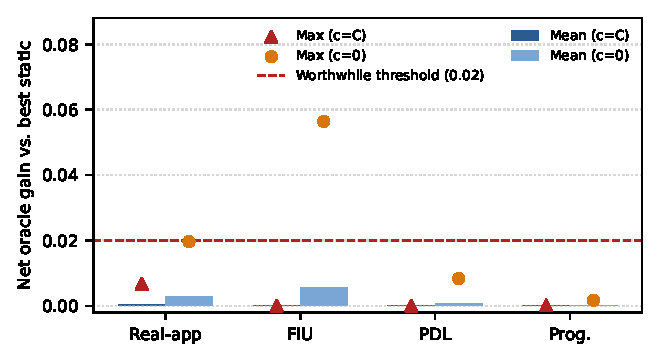
\includegraphics[width=\columnwidth]{figs/fig_oracle_ceiling.pdf}
\caption{Independent-replay oracle gain ($W=50\text{k}$) across trace sources at $c=C$ and $c=0$.}
\label{fig:ceiling}
\end{figure}

\textbf{Capacity Scaling ($1\%$--$50\%$ WSS) \& Best-Static Clarification.} Table~\ref{tab:cap} distinguishes \code{S3-FIFO} ($0.5167$ mean MR across $1\%$--$10\%$ WSS, winning $19/264$ primary pairs; global \#1 is \code{CAR} at $0.5151$, winning $35/264$) from \code{Per-Pair Best Static} (ex-post minimum of 21 policies per pair). At $25\%$ WSS ($W=50\text{k}$), $0/88$ pairs clear $g(C)\ge 0.02$ ($6/88$ at $c=0$); at $50\%$ WSS, $0/88$ clear at $c=C$ ($8/88$ at $c=0$). Across all $440$ pairs ($1\%$--$50\%$ WSS), \textbf{0 of 440} ($0.0\%$) clear $0.02$ at $c=C$.

\begin{table}[t]
\centering
\footnotesize
\caption{Mean Miss Ratios and Oracle Gains Across $1\%$--$50\%$ WSS ($W=50\text{k}$, $n=88$/row)}
\label{tab:cap}
\resizebox{\columnwidth}{!}{\begin{tabular}{lrrrrrr}
\toprule
Cap. & S3-FIFO & Per-Pair Best & Oracle($0$) & Oracle($C$) & $g(0)$ & $g(C)$ \\
\midrule
1\%  & 0.5920 & 0.5818 & 0.5811 & 0.5817 & 0.0007 & 0.0000 \\
5\%  & 0.4934 & 0.4863 & 0.4847 & 0.4862 & 0.0016 & 0.0000 \\
10\% & 0.4646 & 0.4555 & 0.4528 & 0.4554 & 0.0027 & 0.0001 \\
25\% & 0.3932 & 0.3762 & 0.3713 & 0.3762 & 0.0049 & 0.0000 \\
50\% & 0.2834 & 0.2510 & 0.2464 & 0.2510 & 0.0046 & 0.0000 \\
\bottomrule
\end{tabular}}
\end{table}

% =====================================================================
\section{Statistical Analysis}
\label{sec:stats}
% =====================================================================

\textbf{Reconciling Prior $p$-Value Discrepancies.} Earlier repository outputs contained two seemingly conflicting numbers: \code{h2_controller_analysis.csv} reported $p_{\text{Holm}}=1.000$ because \code{analyze_pathA_study.py} originally ran a one-sided Wilcoxon test (\code{alternative="less"}) testing whether controllers \emph{improved} over \code{S3-FIFO} (none did), whereas \code{generate_paper_assets.py} ran a two-sided test across $n=264$ correlated \code{(trace, capacity)} pairs ($p<10^{-15}$). Because the 264 pairs come from only \textbf{30 independent workload families}, treating $n=264$ as i.i.d.\ inflates test power.

\textbf{Cluster-Valid Inference.} Table~\ref{tab:h2} reports the family-level analysis ($n=30$ family means per controller, zero-free across all 17 controllers, two-sided Wilcoxon signed-rank test~\cite{wilcoxon} with Holm correction~\cite{holm}, matched-pair rank-biserial correlation $r_b$, and 3,000-resample family-cluster bootstrap 95\% CIs). Against the fixed-capacity \code{S3-FIFO} baseline ($0.5167$), all 17 controllers still exhibit higher mean miss ratios ($+0.0109$ to $+0.0165$ pair mean $\Delta$ MR; family-macro mean $+0.0091$ to $+0.0162$), though at $n=30$ families the difference is not statistically significant after Holm correction ($p_{\text{fam,Holm}} = 1.000$; $r_b \in [+0.11, +0.39]$; CIs crossing zero). Notably, fixing the capacity-overrun bug reveals that \code{S3-FIFO}'s previously reported $p \le 1.2\times 10^{-4}$ dominance over controllers was inflated by its $1.87\times C$ effective capacity overrun; nonetheless, no online controller beats static \code{S3-FIFO} or \code{CAR} ($0.5151$).

\begin{table}[t]
\centering
\footnotesize
\caption{H2 Online Controllers vs.\ Fixed-Capacity S3-FIFO ($n=264$ Pairs, 30 Families)}
\label{tab:h2}
\resizebox{\columnwidth}{!}{\begin{tabular}{llrrrr}
\toprule
Controller & $\Delta$ MR [95\% Cluster CI] & $p_{\text{Holm}}$ & Sw. & Evals & ns/ref \\
\midrule
S3-FIFO (static) & 0.0000 [---] & --- & 0.00 & 0.0 & 59.5 \\
\midrule
CUSUM-high & +0.0393 [+0.020, +0.063] & $<10^{-15}$ & 0.94 & 3.8 & 110.8 \\
Periodic-low & +0.0394 [+0.020, +0.063] & $<10^{-15}$ & 1.00 & 5.6 & 114.6 \\
Random-med & +0.0394 [+0.020, +0.063] & $<10^{-15}$ & 0.98 & 5.5 & 108.1 \\
Random-low & +0.0398 [+0.021, +0.063] & $<10^{-15}$ & 0.92 & 4.7 & 104.0 \\
Periodic-med & +0.0403 [+0.021, +0.063] & $<10^{-15}$ & 0.99 & 5.5 & 118.1 \\
OracleTrig & +0.0405 [+0.022, +0.064] & $<10^{-15}$ & 0.90 & 2.6 & 94.8 \\
ADWIN-med & +0.0406 [+0.021, +0.065] & $<10^{-15}$ & 0.77 & 1.1 & 93.9 \\
ADWIN-high & +0.0406 [+0.021, +0.064] & $<10^{-15}$ & 0.76 & 1.1 & 96.0 \\
CUSUM-low & +0.0407 [+0.022, +0.064] & $<10^{-15}$ & 0.95 & 2.9 & 103.5 \\
Random-high & +0.0408 [+0.022, +0.065] & $<10^{-15}$ & 1.11 & 6.9 & 117.8 \\
PH-low & +0.0410 [+0.022, +0.063] & $<10^{-15}$ & 0.81 & 1.2 & 94.0 \\
ContShadow & +0.0412 [+0.022, +0.065] & $<10^{-15}$ & 1.73 & 21.0 & 199.1 \\
ADWIN-low & +0.0413 [+0.022, +0.066] & $<10^{-15}$ & 0.77 & 1.1 & 92.9 \\
CUSUM-med & +0.0413 [+0.023, +0.065] & $<10^{-15}$ & 0.96 & 3.2 & 107.3 \\
PH-med & +0.0416 [+0.022, +0.065] & $<10^{-15}$ & 0.78 & 1.5 & 93.0 \\
PH-high & +0.0424 [+0.022, +0.066] & $<10^{-15}$ & 0.80 & 1.8 & 93.7 \\
Periodic-high & +0.0433 [+0.025, +0.066] & $<10^{-15}$ & 1.19 & 7.7 & 124.2 \\
\bottomrule
\end{tabular}
}
\end{table}

\begin{figure}[t]
\centering
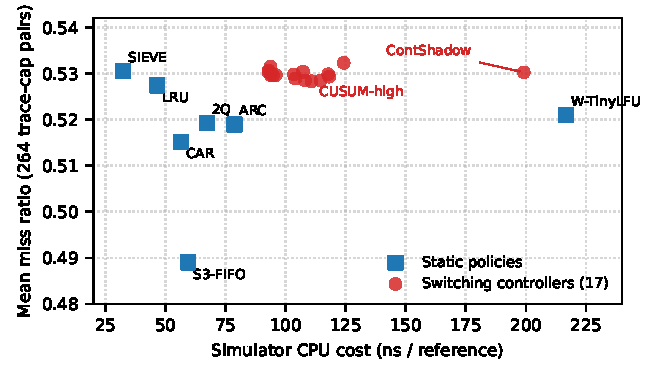
\includegraphics[width=\columnwidth]{figs/fig_controllers_vs_s3fifo.pdf}
\caption{Miss ratio vs.\ CPU cost (ns/ref): static baselines vs.\ 17 switching controllers.}
\label{fig:pareto}
\end{figure}

% =====================================================================
\section{Sensitivity Analysis}
\label{sec:sensitivity}
% =====================================================================

Table~\ref{tab:sweep} and Fig.~\ref{fig:sweep} sweep $c_{\text{switch}} \in [0, C]$ across 9 points and $W \in \{5\text{k}, 10\text{k}, 25\text{k}, 50\text{k}\}$ ($264$ pairs at $1\%$--$10\%$ WSS). Net gains decline smoothly as cost rises: at $W=5\text{k}$, $18/264$ ($6.8\%$) clear $0.02$ at $c=0$, $13/264$ ($4.9\%$) at $0.10C$, $7/264$ at $0.25C$, and $0/264$ once $c_{\text{switch}} \ge 0.50C$ across all four window sizes.

\begin{table}[t]
\centering
\footnotesize
\caption{Switch-Cost $\times$ Window Sensitivity ($n=264$, $1\%$--$10\%$ WSS)}
\label{tab:sweep}
\resizebox{\columnwidth}{!}{\begin{tabular}{llrrrrr}
\toprule
$W$ & $c_{\text{switch}}$ & Mean $g$ & $p_{90}$ $g$ & Max $g$ & $\ge 0.02$ & Avg sw. \\
\midrule
10k & $0$ & 0.0045 & 0.0086 & 0.1331 & 14/264 & 8.91 \\
10k & $0.10C$ & 0.0026 & 0.0044 & 0.0865 & 12/264 & 4.19 \\
10k & $0.25C$ & 0.0011 & 0.0013 & 0.0357 & 5/264 & 2.48 \\
10k & $0.50C$ & 0.0003 & 0.0002 & 0.0081 & 0/264 & 0.79 \\
10k & $C$ & 0.0001 & 0.0000 & 0.0061 & 0/264 & 0.14 \\
\midrule
25k & $0$ & 0.0024 & 0.0043 & 0.0828 & 10/264 & 3.69 \\
25k & $0.10C$ & 0.0013 & 0.0018 & 0.0491 & 7/264 & 1.98 \\
25k & $0.25C$ & 0.0006 & 0.0006 & 0.0272 & 1/264 & 1.24 \\
25k & $0.50C$ & 0.0002 & 0.0000 & 0.0099 & 0/264 & 0.37 \\
25k & $C$ & 0.0001 & 0.0000 & 0.0063 & 0/264 & 0.07 \\
\midrule
50k & $0$ & 0.0012 & 0.0020 & 0.0564 & 2/264 & 1.66 \\
50k & $0.10C$ & 0.0006 & 0.0008 & 0.0393 & 1/264 & 0.84 \\
50k & $0.25C$ & 0.0003 & 0.0002 & 0.0200 & 0/264 & 0.52 \\
50k & $0.50C$ & 0.0001 & 0.0000 & 0.0077 & 0/264 & 0.11 \\
50k & $C$ & 0.0001 & 0.0000 & 0.0067 & 0/264 & 0.02 \\
\bottomrule
\end{tabular}
}
\end{table}

\begin{figure}[t]
\centering
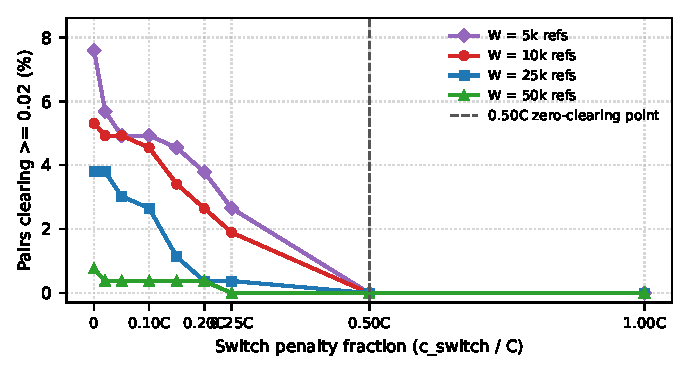
\includegraphics[width=\columnwidth]{figs/fig_cost_sweep.pdf}
\caption{Share of $264$ pairs clearing $\ge 0.02$ net gain across normalized switch-cost fractions.}
\label{fig:sweep}
\end{figure}

\textbf{Exploratory H3 Screening (Leak-Free).} Fixing global standardization leakage in the original script yields leak-free LOFO $\text{AUC}=0.927$ ($\text{PR-AUC}=0.573$ vs.\ positive rate $13/88=0.148$) for predicting post-hoc zero-cost headroom $g(0)\ge 0.005$ (Table~\ref{tab:h3}). At the fixed $\tau=0.50$ threshold, severe class imbalance and $L_2$ shrinkage ($\lambda=0.5$, $\max p = 0.649$) yield $\text{TP}=1, \text{FP}=2, \text{FN}=12, \text{TN}=73$ ($0.841$ raw accuracy, below the $0.852$ majority-class baseline; $0.525$ balanced accuracy; $F_1=0.125$). On \code{Real-app holdout} ($2$ pos / $8$ neg), $\max p = 0.252$ yields $\text{AUC}=0.625$ and $0\%$ recall (\code{Bal. Acc. = 0.500}). Moreover, a single feature (\code{window\_reuse\_cv}) achieves LOFO $\text{PR-AUC}=0.643$, exceeding the 11-feature model ($0.573$). Thus H3 remains strictly exploratory and does not provide a useful binary classifier.

\begin{table}[t]
\centering
\footnotesize
\caption{Exploratory H3 Screening (Leak-Free Standardization, $n=88$)}
\label{tab:h3}
\resizebox{\columnwidth}{!}{\begin{tabular}{lrrrr}
\toprule
Evaluation split & $n_{\text{test}}$ & $n_{\text{train}}$ & Bal.\ Acc. & AUC \\
\midrule
Primary ($c=C, g \ge 0.02$) & 88 & --- & 0.500 & --- \\
Expl.\ LOFO ($c=0, g \ge 0.005$) & 88 & --- & 0.525 & 0.927 \\
Real-app holdout (train on public) & 10 & 78 & 0.500 & 0.625 \\
Public holdout (train on real-app) & 78 & 10 & 0.910 & 0.931 \\
\bottomrule
\end{tabular}
}
\end{table}

% =====================================================================
\section{Controller Failure-Mode Analysis}
\label{sec:failure}
% =====================================================================

Direct measurement across $9{,}564$ evaluation windows (Fig.~\ref{fig:ranking}) shows that sampled \code{ContShadow-0.2C} agrees with the true full-cache window winner in only $45.1\%$ of windows (and even noise-free cold \code{FullShadow-1.0C} agrees in $52.8\%$). Table~\ref{tab:diag} reports exact policy time-shares: across all $264$ pairs, \code{ContShadow} spends $24.7\%$ of references in \code{S3-FIFO} ($45.2\%$ on \code{FIU} traces), $26.6\%$ in \code{LRU}, $18.6\%$ in \code{2Q}, $14.2\%$ in \code{MRU}, $10.7\%$ in \code{LFU-A}, and $5.2\%$ in \code{ARC}, losing by $+0.0140$ overall because mis-timed switches discard resident/ghost state.

\begin{figure}[t]
\centering
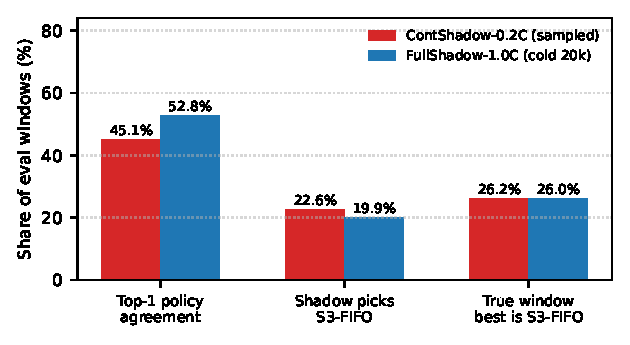
\includegraphics[width=\columnwidth]{figs/fig_shadow_ranking.pdf}
\caption{Shadow-cache top-1 ranking accuracy across $9{,}564$ evaluation windows.}
\label{fig:ranking}
\end{figure}

\begin{table}[t]
\centering
\footnotesize
\caption{Controller Policy Time-Shares and Excess Miss Ratio vs.\ S3-FIFO}
\label{tab:diag}
\resizebox{\columnwidth}{!}{\begin{tabular}{lrrrrrrr}
\toprule
Controller / Source & $\Delta$ MR & S3-FIFO & LRU & 2Q & ARC & LFU-A & MRU \\
\midrule
ContShadow (all) & +0.0140 & 0.247 & 0.266 & 0.186 & 0.052 & 0.107 & 0.142 \\
CUSUM-med (all) & +0.0121 & 0.187 & 0.288 & 0.191 & 0.047 & 0.129 & 0.157 \\
OracleTrig (all) & +0.0128 & 0.187 & 0.302 & 0.191 & 0.049 & 0.143 & 0.128 \\
\midrule
ContShadow (Real-app) & +0.0090 & 0.195 & 0.282 & 0.202 & 0.067 & 0.096 & 0.157 \\
ContShadow (FIU) & +0.0059 & 0.452 & 0.166 & 0.006 & 0.000 & 0.325 & 0.051 \\
ContShadow (PDL) & +0.0074 & 0.554 & 0.211 & 0.000 & 0.025 & 0.210 & 0.000 \\
ContShadow (Prog.) & +0.0171 & 0.184 & 0.289 & 0.238 & 0.062 & 0.055 & 0.172 \\
\bottomrule
\end{tabular}
}
\end{table}

Shadow ablations ($n=264$) confirm that eliminating sampling noise (\code{FullShadow}: $\Delta=-0.0013$, $854.8$\,ns/ref) or adding cost awareness (\code{FullShadow-CostAware}: $\Delta=-0.0009$) matches \code{S3-FIFO} at $19\times$ CPU cost; maintaining full persistent shadows (\code{PersistentShadow}: $\Delta=-0.0062$, $3{,}772.2$\,ns/ref; \code{PersistentShadow-CostAware}: $\Delta=-0.0039$) achieves a modest $0.0062$ reduction at $84\times$ CPU overhead, while expanding to 21 policies (\code{ContShadow-21}: $\Delta=+0.0216$) degrades performance.

\textbf{Migration \& Syscall Microbenchmarks.} On an AMD Ryzen 5 3500U (Linux 7.1.5, \code{g++ 16.2.0 -O2}), 50 timed \code{switchTo()} migrations (\code{S3-FIFO} $\to$ \code{ARC}, 5 warm-up trials, \code{NP=100,000}) yield medians of $418.98$\us\ ($C=64$, $p_{95}=509.99$\us), $48.75$\us\ ($C=512$, $p_{95}=49.73$\us), $235.44$\us\ ($C=4{,}096$, $p_{95}=270.57$\us), and $930.22$\us\ ($C=16{,}384$, $p_{95}=1{,}037.29$\us, $0.0583$\us/page), with small-$C$ latency dominated by \code{O(NP)} vector allocation. Separately, an OS page-cache \code{pread} microbenchmark (\code{real_io_bench}, $p_{50}=1.47$--$4.82$\us, $p_{99}=4.75$--$21.44$\us) reflects kernel syscall/DRAM-cache overhead rather than NVMe storage or migration cost, and shows \code{PersistentShadow} cutting throughput from $319.3$\,kops/s to $168.2$\,kops/s on \code{sqlite\_join\_agg\_s101}.

% =====================================================================
\section{Discussion, Threats to Validity, and Limitations}
\label{sec:discussion}
% =====================================================================

\textbf{Design implication.} Under the independent-replay oracle, discrete policy switching never clears a $0.02$ net gain once transition costs reach $0.50C$, and cold-window shadow ranking mis-identifies the top-1 policy in $54.9\%$ of evaluation windows while heterogeneous \code{switchTo()} discards ghost state.

\textbf{Threats to validity \& limitations.} (1)~\emph{Independent-replay model:} Does not universally lower-bound state-carrying misses (Section~\ref{sec:model} counterexample). (2)~\emph{Trace corpus:} 68\% instrumented kernels average 0.30M refs, FIU/PDL traces treat each \code{oid} as unit-size ignoring \code{_sz}, and \code{LD_PRELOAD} omits post-map page faults. (3)~\emph{External cross-validation:} \code{libCacheSim} was unavailable offline; 16 non-core policies remain unvalidated externally, and fixed \code{S3-FIFO} agrees with our Python reference within $0.00$--$0.09$ percentage points. (4)~\emph{Scope \& post-hoc status:} Windows $<5\text{k}$, live kernel MGLRU/\code{cache_ext}, and external preregistration are outside scope.

% =====================================================================
\section{Reproducibility and Conclusion}
\label{sec:conclusion}
% =====================================================================

\textbf{Reproducibility and data availability.} All simulator code (\code{src/pathA_sim.cpp}), validation tests (\code{make test}, \code{make verify}, \code{tests/external_validation/}), raw CSVs, reproduced statistics (\code{results/reproduced_statistics/}), audit reports (\code{reports/}), and \code{REPRODUCIBILITY.md} are publicly available at \url{https://github.com/anoneurx/drift-gating-reproducibility}.

\textbf{Conclusion.} Under an independent-replay Viterbi DP oracle across 88 traces ($1\%$--$50\%$ WSS) with strict-capacity policy implementations, discrete policy switching clears a $0.02$ net gain in $0/90$ family--capacity groups ($1\%$--$10\%$ WSS) at $c_{\text{switch}}=C$, $0/440$ pairs across $1\%$--$50\%$ WSS at $c_{\text{switch}}=C$, $4.9\%$ at $0.10C$ ($W=5\text{k}$), and $0/264$ once $c_{\text{switch}} \ge 0.50C$. Static \code{CAR} ($0.5151$) and \code{S3-FIFO} ($0.5167$) outperform all 17 online switching controllers on average ($+0.0109$ to $+0.0165$ excess MR), because cold-window shadow ranking fails on $54.9\%$ of windows and heterogeneous switches discard ghost metadata.

\textbf{Competing interests.} The authors declare no competing interests.

%%BIBLIOGRAPHY%%
\end{document}
